\documentclass[11pt,a4paper]{article}
\usepackage[T1]{fontenc}
\usepackage{lmodern}
\usepackage[latin1]{inputenc}
\usepackage{a4wide}
\usepackage[dvips]{graphicx}
\usepackage{float}

\usepackage[
pdfauthor={ace project team},
pdftitle={Final Report},
pdfcreator={pdftex},
]{hyperref}

\usepackage{sectsty}
\allsectionsfont{\sffamily}

\usepackage{fancyheadings} 
\pagestyle{fancy} 
\lhead{\textsf{\textbf{ACE} \\ \small{a collaborative editor}}}
\chead{}
\rhead{
\parbox[c]{3cm}{
\includegraphics[height=0.875cm,width=3cm]{../../images/logo_BFH.eps}}
\parbox[c]{2.2cm}
{\tiny{\textsf{Berner Fachhochschule \\
Hochschule f�r \\
Technik und Informatik}}}}
\lfoot{}
\cfoot{\textsf{\thepage}}
\rfoot{}
\setlength{\headrulewidth}{0.6pt}
\setlength{\footrulewidth}{0.6pt}
\setlength{\topmargin}{-50pt}
\addtolength{\headheight}{50pt}

\usepackage{colortbl}

\newcommand{\headercol}[2]{\multicolumn{1}{|>{\bfseries\columncolor[gray]{0.82}}p{#1}|}{\textsf{#2}}}
\newcommand{\ace}[0]{\emph{ACE }}



\begin{document}
\setlength{\parindent}{0pt}

\begin{titlepage}
\thispagestyle{empty}
  
\includegraphics[height=1.5in]{../images/pix.eps}

  \begin{center}

    {\fontsize{40}{45} \textbf{\textsf{ACE}}} \\
    \textsf{a collaborative editor} \\
        
    \vspace{36pt}
        
    {\huge{\textbf{\textsf{}}}} \\

    \vspace{36pt}

	\textsf{Berne University of Applied Sciences} \\
    \textsf{School of Engineering and Information Technology} \\
    
  \end{center}

  \vfill
  
  \begin{tabular}{ll}
   \hline

   \\

   \multicolumn{1}{>{\bfseries}p{1.5in}}{\textsf{Date:}} &
   \multicolumn{1}{>{}p{4.3in}}{\textsf{08.11.2005}}          \\
   
   \\
   
   \multicolumn{1}{>{\bfseries}p{1.5in}}{\textsf{Version:}}     &   
   \multicolumn{1}{>{}p{4.3in}}{\textsf{0.1}}                 \\

   \\
   
   \multicolumn{1}{>{\bfseries}p{1.5in}}{\textsf{Projectteam:}}                 &
   \multicolumn{1}{>{}p{4.3in}}{\textsf{Mark Bigler (biglm2@hta-bi.bfh.ch)}}  \\
   \multicolumn{1}{>{\bfseries}p{1.5in}}{}                                      &
   \multicolumn{1}{>{}p{4.3in}}{\textsf{Simon Raess (rasss@hta-bi.bfh.ch)}}    \\
   \multicolumn{1}{>{\bfseries}p{1.5in}}{}                                      &
   \multicolumn{1}{>{}p{4.3in}}{\textsf{Lukas Zbinden (zbinl@hta-bi.bfh.ch)}} \\   
   
   \\
   
   \multicolumn{1}{>{\bfseries}p{1.5in}}{\textsf{Receivers:}}                       &
   \multicolumn{1}{>{}p{4.3in}}{\textsf{Jean-Paul Dubois (doj@hta-bi.bfh.ch)}}       \\
   \multicolumn{1}{>{\bfseries}p{1.5in}}{}                                          &
   \multicolumn{1}{>{}p{4.3in}}{\textsf{Claude Fuhrer (frc@hta-bi.bfh.ch)}}       \\

   \\
   
   \multicolumn{1}{>{\bfseries}p{1.5in}}{\textsf{Location:}}               &   
   \multicolumn{1}{>{}p{4.3in}}{\textsf{Subversion Repository}} \\

   \\  
   
   \hline
  \end{tabular}

\end{titlepage}

\newpage

\tableofcontents
\newpage

\listoftables
\listoffigures
\newpage


\section{Introduction}
\subsection{Purpose}
The purpose of this document is to give a general overview of all the available documents, the achieved results and to make a brief outlook.

\subsection{Referenced Documents}
All the referenced documents can be found on the project website (\href{http://ace.iserver.ch/}{http://ace.iserver.ch/}) or in the subversion repository (\href{http://ace.iserver.ch:81/repos/ace/ace/}{http://ace.iserver.ch:81/repos/ace/ace/}).

\paragraph{PM Documents}
\begin{itemize}
 \item \href{http://ace.iserver.ch:81/repos/ace/ace/trunk/doc/pdf/projectmanual.pdf}{Project Manual}
 \item \href{http://ace.iserver.ch:81/repos/ace/ace/trunk/doc/pdf/projektplan.pdf}{Project Plan}
 \item \href{http://ace.iserver.ch:81/repos/ace/ace/trunk/doc/pdf/erfahrungsbericht.pdf}{Final Report PM}
\end{itemize}

\paragraph{Documentation}
\begin{itemize}
 \item \href{http://ace.iserver.ch:81/repos/ace/ace/trunk/doc/pdf/algorithm.pdf}{Report Evaluation Algorithms}
 \item \href{http://ace.iserver.ch:81/repos/ace/ace/trunk/doc/pdf/implementation-algorithm.pdf}{Report Implementation Algorithm}
 \item \href{http://ace.iserver.ch:81/repos/ace/ace/trunk/doc/pdf/testframework.pdf}{Report Implementation Testframework}
 \item \href{http://ace.iserver.ch:81/repos/ace/ace/trunk/doc/pdf/network.pdf}{Report Evaluation Network}
 \item \href{http://ace.iserver.ch:81/repos/ace/ace/trunk/doc/pdf/gui.pdf}{Report Evaluation GUI}
\end{itemize}


\section{Project}
The planned project organization and phases are described in the project plan and project manual.

\subsection{Phases}
The project was split into three distinct phases: initialization, construction, and termination. The construction phase was split into three independent subprojects: algorithm, network, and GUI. The lifecycle model is depicted in figure \ref{fig:lifecycle}.

\begin{figure}[H]
 \centering
 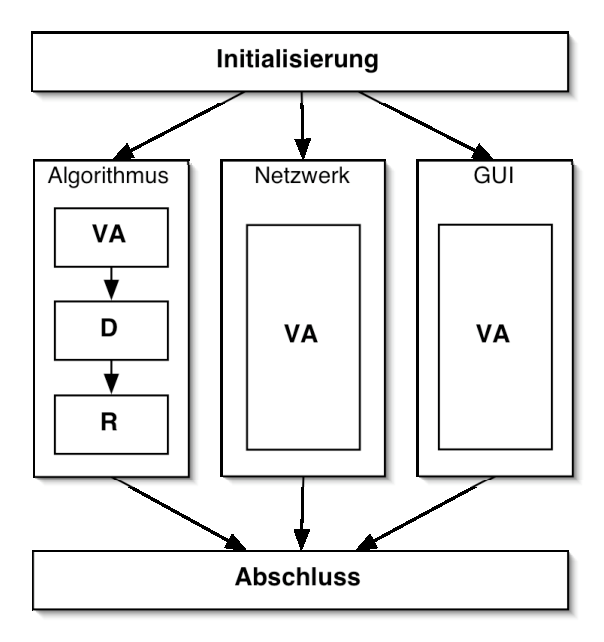
\includegraphics[width=8cm,height=8.5cm]{../../images/vorgehensmodell.eps}
 \caption{Lifecycle Model used in Semester Project}
 \label{fig:lifecycle}
\end{figure}

\subsection{Decisions}
The following decisions have been made:
\begin{itemize}
 \item algorithm: Jupiter
 \item resulting from the above point: client-server architecture
\end{itemize}
Several decisions are deliberately left open:
\begin{itemize}
 \item Which network technologies do we use for implementation of network layer?
 \item Will the concurrency control algorithm be integrated into an existing application (for instance \emph{JEdit}) or will we develop a standalone application?
\end{itemize}
Further, we have decided to continue the project as our diploma project.

\subsection{Results}
The expected results are described in the project plan. In the following sections all the major documents are presented. These documents are the source of all the information about the project itself.

\subsubsection{Algorithm}
\paragraph{Report Evaluation Algorithms:} 
This report describes the core principles of collaborative editing, evaluates several algorithms and proposes a few algorithms for a possible implementation.

\paragraph{Report Implementation Algorithm:} 
This report describes which algorithm we chose in great detail. Also a justification for our selection is given.

\paragraph{Report Implementation Testframework:}
This report describes the testframework and shows how one can define testcases (so called scenarios) for the testframework.

\subsubsection{Network}
\paragraph{Report Evaluation Network:}
This report describes the requirements a network layer of \ace must fulfill. It further describes some available network technologies and explains whether they are suitable. A set of selection criteria is given in the \emph{conclusions} of this report.

\subsubsection{GUI}
\paragraph{Report Evaluation GUI:}
The evaluation report GUI describes several key problems that must be solved in the graphical user interface of \ace.


\section{Status}
The goals as described in the project manual are all achieved. However, the implementation of undo in the algorithm still has some flaws. Although we have a complete understanding how to solve these problems, the solution is not yet implemented.

See the \emph{report implementation algorithm} for a description of the remaining issues in the implementation of undo/redo.


\section{Outlook}
We achieved the main objectives of the semester project. We have built a good and solid foundation for a collaborative application. Now, we would like to make a brief outlook for the time up to the diploma project and also for the diploma project itself.

\subsection{Summer}
\begin{itemize}
 \item complete implementation and refactoring of algorithm (undo/redo)
 \item selection of network technology
 \item GUI: integrated in existing application or standalone application?
\end{itemize}

\subsection{Diploma Project}
The implementation of a collaborative text editor will be the main goal of the diploma project. This goal includes several other goals that are needed for a fully functioning application.
\begin{itemize}
 \item network layer (discovery of available shared documents, communication)
 \item GUI: integration of algorithm, sharing of documents, discovery of shared documents
\end{itemize}

\section{Conclusion}
First of all, we used the chance of the semester project to build a solid base for our diploma project. This gave us the chance to collect important experience without the pressure existing in a real world situation. It was generally a very interesting project and a pleasure to work on it.

\end{document}

